\documentclass{jlreq}
\usepackage[dvipdfmx]{graphicx}
\usepackage[dvipdfmx]{color}
\usepackage[dvipdfmx]{hyperref}
\usepackage{amsmath}
\usepackage{geometry}
\usepackage{float}
\usepackage{array}
\usepackage{caption}
\usepackage{hyperref}
\usepackage{url}
\usepackage{listings}
\renewcommand{\lstlistingname}{リスト}
\linespread{1.2}
\numberwithin{equation}{section}
\counterwithin{figure}{section}
\counterwithin{table}{section}
\ModifyHeading{section}{before_space=20pt, after_space=20pt}
\ModifyHeading{subsubsection}{before_space=15pt, after_space=20pt}
\lstset{
    basicstyle = {\ttfamily}, % 基本的なフォントスタイル
    frame = {tbrl}, % 枠線の枠線。t: top, b: bottom, r: right, l: left
    breaklines = true, % 長い行の改行
    showspaces = false, % スペースの表示
    showstringspaces = false, % 文字列中のスペースの表示
    showtabs = false, % タブの表示
    numbers = left, % 行番号の表示。left, right, none
    keywordstyle = \color{blue}, % キーワードのスタイル。intやwhileなど
    commentstyle = {\color[HTML]{1AB91A}}, % コメントのスタイル
    identifierstyle = \color{black}, % 識別子のスタイル 関数名や変数名
    captionpos = t % キャプションの位置 t: 上、b: 下
}

\begin{document}

\section{目的}
ハードウェア記述言語VHDLを用いて、ストップウオッチの機能あるいは回路構成を記述し、それをFPGA上に実現することにより、ディジタル回路の動作原理ならびにその設計手順を理解する。また、設計・シミュレーション・実機検証の一連の工程を通じて、FPGA開発の実践的なスキルを習得し、効率的なデバッグ手法や設計の最適化についても学ぶ。

\section{原理}
\subsection{FPGAの原理}
FPGA(Field Programmable Gate Array)は、ユーザーが回路構成を自由に書き換えられる集積回路である。FPGA内部には多数のロジックブロック(論理素子)と、それらを相互接続する配線(インターコネクト)、そして設定情報を保持する構成メモリが組み込まれている。ユーザーはHDL(ハードウェア記述言語)を使って回路設計を行い、そのデータをFPGAに書き込むことで、加算器やカウンタ、プロセッサなど多様なデジタル回路を構成することができる。これにより、専用ICのようなハードウェアの高速性と、ソフトウェアの柔軟性を両立できる。(1)

FPGAのチップの内では、論理機能を実現することができ、EmbeddedArrayBlock(EAB)およびLogicArrayBlock(LAB)、ならびにそれらを接続するためのFastTrack列配線および行配線が、図2.1に示すように規則的に配置されている。

\begin{figure}[H]
  \centering
  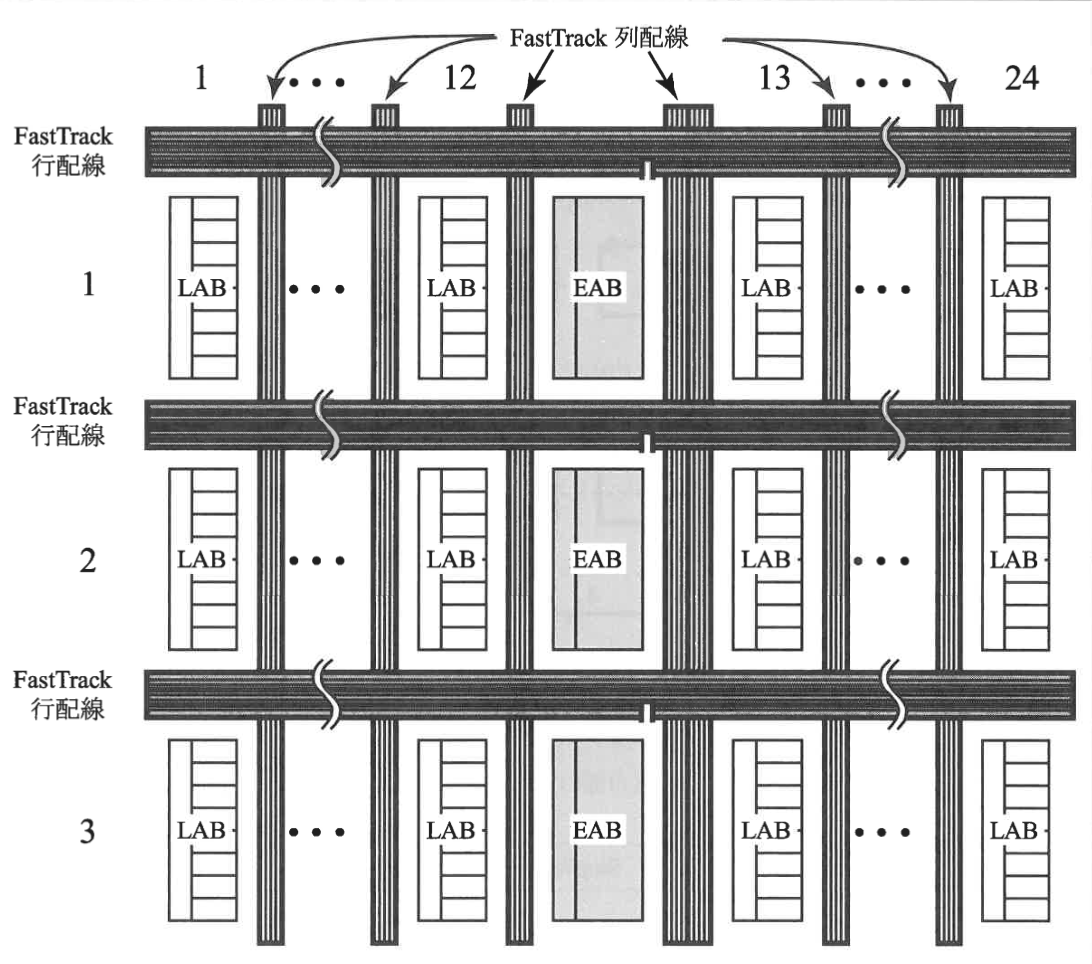
\includegraphics[width=0.7\textwidth]{assets/EP1K10_stracture.png}
  \caption{EP1K10の構造}
\end{figure}

EP1K10は3行25列構造で、各行にEABが1個、LABが24個配置されている。FastTrack配線は高速伝送が可能で、行配線は144本、列配線は通常24本だが、EAB横は48本となっている。EABは8入力16出力の任意関数を実現可能で、RAMやFIFOなどのメモリ機能やデータ処理にも利用できる。例えば、1つのEABで256x16ビットや512x8ビットのRAMを構成可能で、複数のEABを組み合わせることでより大容量のRAMも実現できる。

\subsection{実験で作成したstop watchのモジュール構成と動作原理}

\section{実験結果}

\subsection{実験手順}

\subsubsection{VHDLコードの作成}
サブモジュールである周期0.1秒のパルス発生回路(PulseGen01)をVHDLで記述し、PulseGen01.vhd)として作成する。

\subsubsection{コンパイルとデバッグ}
Quartus Primeを用いてVHDLコードをコンパイルし、FPGA(MAX10 10M50)に実装可能な回路へ変換する。コンパイル時にエラーが発生した場合は、デバッグを行い記述を修正する。

\subsubsection{シミュレーションによる動作確認}
Quartus Primeのシミュレーション機能を利用して、設計した回路が仕様通り動作するか確認する。問題があれば再度デバッグを行う。

\subsubsection{FPGAへの書き込みとボード上での実機動作確認}
動作が確認できた後、回路データをMAX10 10M50ボードへダウンロードし、実際のハードウェア上で動作を確認する。

\lstinputlisting[caption=PulseGen01.vhd, label=code:ext, language=VHDL]{PulseGen01.vhd}

\section{実験結果}

\subsection{使用機材}

\subsection{参考文献}
\begin{enumerate}
  \item FPGAとは, フィールドでプログラムできる論理回路 \\
    \url{https://jp.mathworks.com/discovery/fpga.html}\\
    閲覧日:2025年5月21日
\end{enumerate}

\end{document}